\documentclass[aspectratio=169]{beamer}
\usetheme{Madrid}
\usecolortheme{default}

\usepackage{graphicx}
\usepackage{listings}
\usepackage{xcolor}
\usepackage{amsmath}
\usepackage{tikz}
\usepackage{url}

% Code listing setup
\lstset{
    basicstyle=\ttfamily\scriptsize,
    keywordstyle=\color{blue}\bfseries,
    commentstyle=\color{green!60!black},
    stringstyle=\color{red},
    breaklines=true,
    frame=single,
    backgroundcolor=\color{gray!10},
    language=Python
}

\title{Dask DataFrames}
\subtitle{Parallel Pandas for Large Datasets}
\author{CSE255 - Scalable Data Analysis}
\date{\today}

\begin{document}

\frame{\titlepage}

\begin{frame}{DataFrame Architecture}
\small
\begin{itemize}
    \item One Dask DataFrame = many pandas DataFrames
    \item Partitioned along index
    \item Each partition is a pandas DataFrame
    \item Operations applied to each partition in parallel
\end{itemize}

\vspace{0.1cm}
\textbf{Key Insight:}
\begin{itemize}
    \item Think of Dask DataFrame as a "meta-DataFrame"
    \item Contains references to many pandas DataFrames
    \item Each partition can be on different machines
\end{itemize}
\end{frame}

\begin{frame}[fragile]{Blocked Parallel Strategy}
\small
\textbf{How It Works:}
\begin{enumerate}
    \item Data split into blocks (partitions)
    \item Operations applied to each block independently
    \item Results combined to form final answer
\end{enumerate}

\vspace{0.15cm}
\textbf{Example:}
\begin{itemize}
    \item 1TB dataset $\rightarrow$ 10 partitions of 100GB each
    \item Each partition processed in parallel
    \item Results merged at the end
\end{itemize}
\end{frame}

\begin{frame}{Blocked Parallel Strategy: Visualization}
\begin{center}
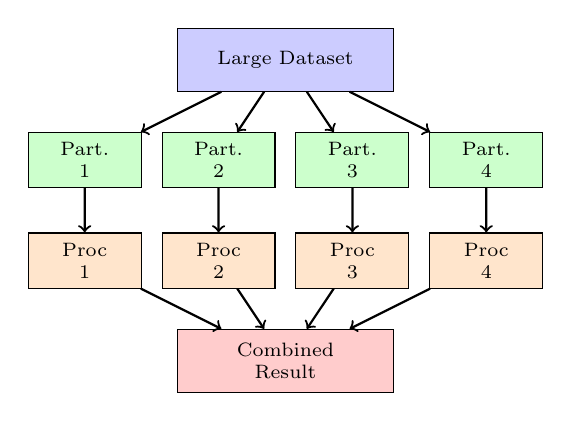
\begin{tikzpicture}[node distance=1.2cm, auto, scale=0.85, every node/.style={font=\scriptsize}]
    % Large Dataset - positioned at top center
    \node[draw, rectangle, fill=blue!20, text width=2.5cm, align=center, minimum height=0.8cm] (dataset) at (0,3) {Large Dataset};
    
    % Partitions - spread out horizontally with more space
    \node[draw, rectangle, fill=green!20, text width=1.2cm, align=center, minimum height=0.7cm] (p1) at (-3,1.5) {Part.\\1};
    \node[draw, rectangle, fill=green!20, text width=1.2cm, align=center, minimum height=0.7cm] (p2) at (-1,1.5) {Part.\\2};
    \node[draw, rectangle, fill=green!20, text width=1.2cm, align=center, minimum height=0.7cm] (p3) at (1,1.5) {Part.\\3};
    \node[draw, rectangle, fill=green!20, text width=1.2cm, align=center, minimum height=0.7cm] (p4) at (3,1.5) {Part.\\4};
    
    % Processes - aligned with partitions, more vertical space
    \node[draw, rectangle, fill=orange!20, text width=1.2cm, align=center, minimum height=0.7cm] (proc1) at (-3,0) {Proc\\1};
    \node[draw, rectangle, fill=orange!20, text width=1.2cm, align=center, minimum height=0.7cm] (proc2) at (-1,0) {Proc\\2};
    \node[draw, rectangle, fill=orange!20, text width=1.2cm, align=center, minimum height=0.7cm] (proc3) at (1,0) {Proc\\3};
    \node[draw, rectangle, fill=orange!20, text width=1.2cm, align=center, minimum height=0.7cm] (proc4) at (3,0) {Proc\\4};
    
    % Combined Result - centered at bottom
    \node[draw, rectangle, fill=red!20, text width=2.5cm, align=center, minimum height=0.8cm] (result) at (0,-1.5) {Combined\\Result};
    
    % Edges - from dataset to partitions
    \draw[->, thick] (dataset) -- (p1);
    \draw[->, thick] (dataset) -- (p2);
    \draw[->, thick] (dataset) -- (p3);
    \draw[->, thick] (dataset) -- (p4);
    
    % Edges - from partitions to processes
    \draw[->, thick] (p1) -- (proc1);
    \draw[->, thick] (p2) -- (proc2);
    \draw[->, thick] (p3) -- (proc3);
    \draw[->, thick] (p4) -- (proc4);
    
    % Edges - from processes to result
    \draw[->, thick] (proc1) -- (result);
    \draw[->, thick] (proc2) -- (result);
    \draw[->, thick] (proc3) -- (result);
    \draw[->, thick] (proc4) -- (result);
\end{tikzpicture}
\end{center}
\end{frame}

\begin{frame}[fragile]{Creating DataFrames: From Files}
\small
\begin{lstlisting}[basicstyle=\ttfamily\tiny]
import dask.dataframe as dd

# Read CSV files
df = dd.read_csv('data/*.csv')

# Read Parquet files
df = dd.read_parquet('s3://bucket/data/*.parquet')
\end{lstlisting}

\vspace{0.1cm}
\textbf{Key Features:}
\begin{itemize}
    \item Supports glob patterns (\texttt{*}, \texttt{?}, \texttt{[...]})
    \item Automatic schema inference
    \item Lazy loading (no data read until \texttt{.compute()})
\end{itemize}
\end{frame}

\begin{frame}{Creating DataFrames: From Files (Process)}
\small
\textbf{What Happens:}
\begin{itemize}
    \item Dask scans file paths
    \item Infers schema from first file
    \item Creates task graph for reading
    \item Data not loaded until needed
\end{itemize}

\vspace{0.2cm}
\textbf{Benefits:}
\begin{itemize}
    \item Fast: No I/O until compute
    \item Flexible: Can read many files
    \item Efficient: Only loads what you need
\end{itemize}
\end{frame}

\begin{frame}[fragile]{Creating DataFrames: From Pandas}
\small
\begin{lstlisting}
import pandas as pd
import dask.dataframe as dd

# Create pandas DataFrame
pandas_df = pd.DataFrame({
    'col1': range(1000),
    'col2': range(1000, 2000)
})

# Convert to Dask DataFrame
dask_df = dd.from_pandas(pandas_df, npartitions=4)
\end{lstlisting}

\textbf{Key Points:}
\begin{itemize}
    \item Convert existing pandas DataFrames
    \item Specify number of partitions
    \item Useful for testing or small-to-medium data
\end{itemize}
\end{frame}

\begin{frame}{Creating DataFrames: From Pandas (Partitioning)}
\small
\textbf{Partitioning:}
\begin{itemize}
    \item \texttt{npartitions=4} splits data into 4 partitions
    \item Each partition is a pandas DataFrame
    \item Index determines how data is split
\end{itemize}

\vspace{0.2cm}
\textbf{When to Use:}
\begin{itemize}
    \item Testing Dask operations
    \item Converting existing pandas workflows
    \item Small-to-medium datasets
\end{itemize}
\end{frame}

\begin{frame}[fragile]{Lazy Evaluation in Action}
\small
\textbf{What "Lazy" Means:}
\begin{itemize}
    \item \texttt{dd.read\_csv()} doesn't load data
    \item Just creates task graph
    \item \texttt{.compute()} triggers actual loading
\end{itemize}

\vspace{0.1cm}
\textbf{Example:}
\begin{lstlisting}[basicstyle=\ttfamily\tiny]
df = dd.read_csv('data/*.csv')  # Instant
print(df)  # Shows metadata only
result = df.sum()  # Still no data loaded
final = result.compute()  # NOW data loaded
\end{lstlisting}
\end{frame}

\begin{frame}{Lazy Evaluation: Visualization}
\small
\begin{center}
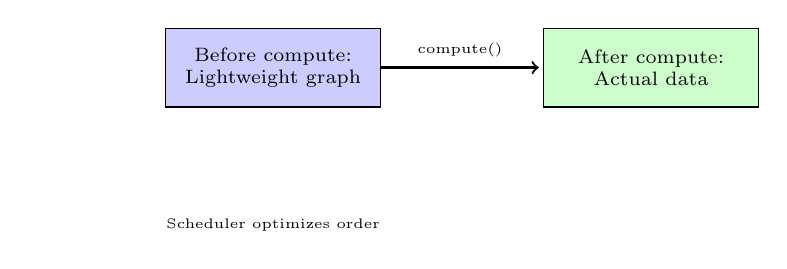
\begin{tikzpicture}[node distance=1.5cm, auto, scale=0.8, every node/.style={font=\scriptsize}]
    % Before compute - positioned explicitly
    \node[draw, rectangle, fill=blue!20, text width=2.5cm, align=center, minimum height=1cm] (before) at (-3,0) {Before compute:\\Lightweight graph};
    
    % Arrow - longer to accommodate spacing
    \draw[->, thick] (before.east) -- ++(2.5,0) node[midway, above, font=\tiny] {compute()};
    
    % After compute - positioned explicitly with more space
    \node[draw, rectangle, fill=green!20, text width=2.5cm, align=center, minimum height=1cm] (after) at (3,0) {After compute:\\Actual data};
    
    % Scheduler note - centered below
    \node[below of=before, yshift=-0.5cm, text width=6cm, align=center, font=\tiny] {Scheduler optimizes order};
\end{tikzpicture}
\end{center}

\vspace{0.2cm}
\textbf{Key Benefit:}
\begin{itemize}
    \item Scheduler can optimize before execution
    \item No wasted computation
    \item Efficient resource usage
\end{itemize}
\end{frame}

\begin{frame}[fragile]{Basic Operations: Inspection}
\small
\begin{lstlisting}
df.head()      # Triggers computation (loads first partition)
df.tail()      # Triggers computation (loads last partition)
df.describe()  # Triggers computation (loads all partitions)
df.dtypes      # No computation needed (metadata)
df.columns     # No computation needed (metadata)
\end{lstlisting}

\textbf{Key Distinction:}
\begin{itemize}
    \item \textbf{Metadata operations}: No computation (fast)
    \item \textbf{Data operations}: Trigger computation (slower)
\end{itemize}

\vspace{0.15cm}
\textbf{When Computation Happens:}
\begin{itemize}
    \item \texttt{.head()}, \texttt{.tail()}: Loads partial data
    \item \texttt{.describe()}, \texttt{len()}: Loads all data
    \item \texttt{.dtypes}, \texttt{.columns}: No data loading
\end{itemize}
\end{frame}

\begin{frame}[fragile]{Filtering and Selection}
\small
\begin{lstlisting}
# Filter rows
filtered = df[df['column'] > 100]

# Select columns
selected = df[['col1', 'col2']]

# Combined
result = df[df['value'] > 50][['col1', 'col2']]
\end{lstlisting}

\textbf{How It Works:}
\begin{itemize}
    \item Works exactly like pandas
    \item Applied to each partition independently
    \item Filtering reduces data size early
\end{itemize}
\end{frame}

\begin{frame}{Filtering and Selection: Visualization}
\small
\begin{center}
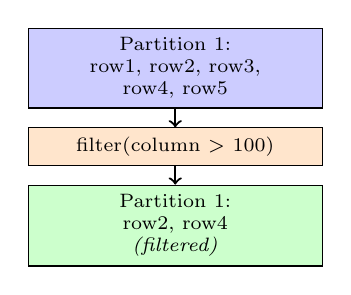
\begin{tikzpicture}[node distance=1cm, auto, scale=0.75, every node/.style={font=\scriptsize}]
    % Input partition
    \node[draw, rectangle, fill=blue!20, text width=3.5cm, align=center] (input) {Partition 1:\\
        row1, row2, row3,\\
        row4, row5};
    
    % Filter operation
    \node[draw, rectangle, fill=orange!20, below of=input, text width=3.5cm, align=center] (filter) {filter(column $>$ 100)};
    
    % Output partition
    \node[draw, rectangle, fill=green!20, below of=filter, text width=3.5cm, align=center] (output) {Partition 1:\\
        row2, row4\\
        \textit{(filtered)}};
    
    % Edges
    \draw[->, thick] (input) -- (filter);
    \draw[->, thick] (filter) -- (output);
\end{tikzpicture}
\end{center}
\end{frame}

\begin{frame}[fragile]{GroupBy Operations: Code}
\small
\begin{lstlisting}
# Group by category
grouped = df.groupby('category')

# Aggregate
result = grouped['value'].sum()
result.compute()

# Multiple aggregations
result = grouped.agg({
    'value': ['sum', 'mean', 'count']
})
\end{lstlisting}

\textbf{Key Features:}
\begin{itemize}
    \item Distributed groupby
    \item Handles shuffles efficiently
    \item Works like pandas groupby
\end{itemize}
\end{frame}

\begin{frame}{GroupBy Operations: Visualization}
\small
\vspace{-0.3cm}
\begin{center}
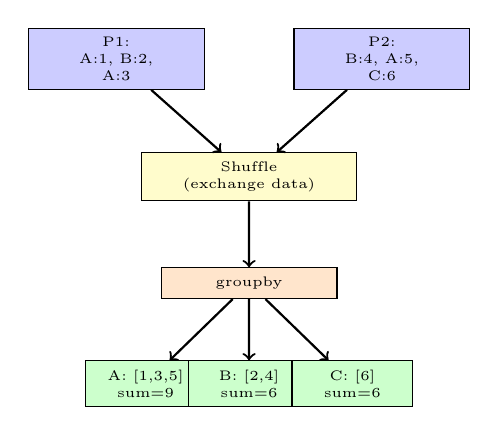
\begin{tikzpicture}[auto, scale=0.75, every node/.style={font=\tiny}]
    % Input partitions - spread out horizontally
    \node[draw, rectangle, fill=blue!20, text width=2cm, align=center] (p1) at (0,0) {P1:\\
        A:1, B:2,\\
        A:3};
    \node[draw, rectangle, fill=blue!20, text width=2cm, align=center] (p2) at (4.5,0) {P2:\\
        B:4, A:5,\\
        C:6};

    % Shuffle step
    \node[draw, rectangle, fill=yellow!20, text width=2.5cm, align=center] (shuffle) at (2.25,-2) {Shuffle\\
        (exchange data)};

    % Groupby operation
    \node[draw, rectangle, fill=orange!20, text width=2cm, align=center] (groupby) at (2.25,-3.8) {groupby};

    % Results - spread out horizontally
    \node[draw, rectangle, fill=green!20, text width=1.3cm, align=center] (a) at (0.5,-5.5) {A: [1,3,5]\\
        sum=9};
    \node[draw, rectangle, fill=green!20, text width=1.3cm, align=center] (b) at (2.25,-5.5) {B: [2,4]\\
        sum=6};
    \node[draw, rectangle, fill=green!20, text width=1.3cm, align=center] (c) at (4,-5.5) {C: [6]\\
        sum=6};

    % Edges from partitions to shuffle
    \draw[->, thick] (p1) -- (shuffle);
    \draw[->, thick] (p2) -- (shuffle);
    
    % Edge from shuffle to groupby
    \draw[->, thick] (shuffle) -- (groupby);
    
    % Edges from groupby to results
    \draw[->, thick] (groupby) -- (a);
    \draw[->, thick] (groupby) -- (b);
    \draw[->, thick] (groupby) -- (c);
\end{tikzpicture}
\end{center}

\vspace{0.1cm}
\footnotesize
\textbf{Note:} Shuffle step moves rows so all rows with same key are together before aggregation.
\end{frame}

\begin{frame}[fragile]{Aggregations: Code}
\small
\begin{lstlisting}
# Column-wise aggregations
df.sum()
df.mean()
df.count()
df.max()
df.min()

# Row-wise aggregations
df.sum(axis=1)
\end{lstlisting}

\textbf{How It Works:}
\begin{itemize}
    \item Applied per partition, then combined
    \item Efficient for large datasets
    \item Same API as pandas
\end{itemize}
\end{frame}

\begin{frame}[fragile]{Aggregations: Example}
\small
\textbf{Example:}
\begin{verbatim}
Partition 1: sum = 100
Partition 2: sum = 200
Partition 3: sum = 150
    | combine
Total sum = 450
\end{verbatim}

\vspace{0.2cm}
\textbf{Process:}
\begin{itemize}
    \item Each partition computes its sum independently
    \item Results are combined to get total
    \item All done in parallel
\end{itemize}
\end{frame}

\begin{frame}[fragile]{Joins and Merges}
\small
\begin{lstlisting}
# Merge two DataFrames
result = dd.merge(df1, df2, on='key')

# Left join
result = dd.merge(df1, df2, on='key', how='left')

# Multiple keys
result = dd.merge(df1, df2, on=['key1', 'key2'])
\end{lstlisting}

\textbf{Key Features:}
\begin{itemize}
    \item Handles large joins efficiently
    \item Partition-aware (optimizes data movement)
    \item Same API as pandas merge
\end{itemize}

\vspace{0.15cm}
\textbf{Performance:}
\begin{itemize}
    \item Dask optimizes join strategy
    \item Minimizes data shuffling
    \item Can handle joins larger than memory
\end{itemize}
\end{frame}

\begin{frame}[fragile]{Pivoting: Long to Wide Tables}
\footnotesize
\textbf{What is Pivoting?}
\begin{itemize}
    \item Transform data from \textbf{long format} (many rows, few columns) to \textbf{wide format} (fewer rows, more columns)
    \item Useful for reshaping data for analysis or visualization
    \item Common operation in data preprocessing
\end{itemize}

\vspace{0.1cm}
\begin{lstlisting}[basicstyle=\tiny]
# Pivot a DataFrame
df_pivot = df.pivot_table(
    index='date',
    columns='category',
    values='value',
    aggfunc='sum'
)

# Alternative: pivot (no aggregation)
df_pivot = df.pivot(
    index='id',
    columns='variable',
    values='value'
)
\end{lstlisting}
\end{frame}

\begin{frame}[fragile]{Pivoting: Visualization}
\begin{center}
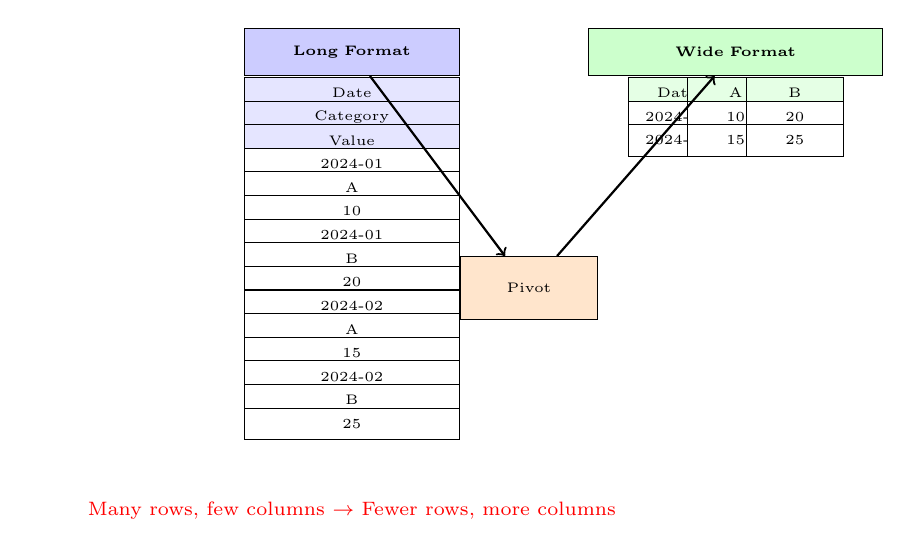
\begin{tikzpicture}[node distance=0.8cm, auto, scale=0.75, every node/.style={font=\tiny}]
    % Long/Thin Table (Input)
    \node[draw, rectangle, fill=blue!20, text width=2.5cm, align=center, minimum height=0.6cm] (long_title) at (-3,2) {\textbf{Long Format}};
    
    \node[draw, rectangle, fill=blue!10, text width=2.5cm, align=center, minimum height=0.4cm] (long_h1) at (-3,1.3) {Date};
    \node[draw, rectangle, fill=blue!10, text width=2.5cm, align=center, minimum height=0.4cm] (long_h2) at (-3,0.9) {Category};
    \node[draw, rectangle, fill=blue!10, text width=2.5cm, align=center, minimum height=0.4cm] (long_h3) at (-3,0.5) {Value};
    
    \node[draw, rectangle, fill=white, text width=2.5cm, align=center, minimum height=0.4cm] (r1_1) at (-3,0.1) {2024-01};
    \node[draw, rectangle, fill=white, text width=2.5cm, align=center, minimum height=0.4cm] (r1_2) at (-3,-0.3) {A};
    \node[draw, rectangle, fill=white, text width=2.5cm, align=center, minimum height=0.4cm] (r1_3) at (-3,-0.7) {10};
    
    \node[draw, rectangle, fill=white, text width=2.5cm, align=center, minimum height=0.4cm] (r2_1) at (-3,-1.1) {2024-01};
    \node[draw, rectangle, fill=white, text width=2.5cm, align=center, minimum height=0.4cm] (r2_2) at (-3,-1.5) {B};
    \node[draw, rectangle, fill=white, text width=2.5cm, align=center, minimum height=0.4cm] (r2_3) at (-3,-1.9) {20};
    
    \node[draw, rectangle, fill=white, text width=2.5cm, align=center, minimum height=0.4cm] (r3_1) at (-3,-2.3) {2024-02};
    \node[draw, rectangle, fill=white, text width=2.5cm, align=center, minimum height=0.4cm] (r3_2) at (-3,-2.7) {A};
    \node[draw, rectangle, fill=white, text width=2.5cm, align=center, minimum height=0.4cm] (r3_3) at (-3,-3.1) {15};
    
    \node[draw, rectangle, fill=white, text width=2.5cm, align=center, minimum height=0.4cm] (r4_1) at (-3,-3.5) {2024-02};
    \node[draw, rectangle, fill=white, text width=2.5cm, align=center, minimum height=0.4cm] (r4_2) at (-3,-3.9) {B};
    \node[draw, rectangle, fill=white, text width=2.5cm, align=center, minimum height=0.4cm] (r4_3) at (-3,-4.3) {25};
    
    % Arrow
    \node[draw, rectangle, fill=orange!20, text width=1.5cm, align=center, minimum height=0.8cm] (pivot_op) at (0,-2) {Pivot};
    
    % Wide Table (Output)
    \node[draw, rectangle, fill=green!20, text width=3.5cm, align=center, minimum height=0.6cm] (wide_title) at (3.5,2) {\textbf{Wide Format}};
    
    \node[draw, rectangle, fill=green!10, text width=1cm, align=center, minimum height=0.4cm] (wide_h1) at (2.5,1.3) {Date};
    \node[draw, rectangle, fill=green!10, text width=1cm, align=center, minimum height=0.4cm] (wide_h2) at (3.5,1.3) {A};
    \node[draw, rectangle, fill=green!10, text width=1cm, align=center, minimum height=0.4cm] (wide_h3) at (4.5,1.3) {B};
    
    \node[draw, rectangle, fill=white, text width=1cm, align=center, minimum height=0.4cm] (wr1_1) at (2.5,0.9) {2024-01};
    \node[draw, rectangle, fill=white, text width=1cm, align=center, minimum height=0.4cm] (wr1_2) at (3.5,0.9) {10};
    \node[draw, rectangle, fill=white, text width=1cm, align=center, minimum height=0.4cm] (wr1_3) at (4.5,0.9) {20};
    
    \node[draw, rectangle, fill=white, text width=1cm, align=center, minimum height=0.4cm] (wr2_1) at (2.5,0.5) {2024-02};
    \node[draw, rectangle, fill=white, text width=1cm, align=center, minimum height=0.4cm] (wr2_2) at (3.5,0.5) {15};
    \node[draw, rectangle, fill=white, text width=1cm, align=center, minimum height=0.4cm] (wr2_3) at (4.5,0.5) {25};
    
    % Edges
    \draw[->, thick] (long_title) -- (pivot_op);
    \draw[->, thick] (pivot_op) -- (wide_title);
    
    % Note
    \node[below of=r4_3, yshift=-0.3cm, text width=8cm, align=center, font=\scriptsize, text=red] {Many rows, few columns $\rightarrow$ Fewer rows, more columns};
\end{tikzpicture}
\end{center}
\end{frame}

\begin{frame}[fragile]{Pivoting: Key Parameters}
\small
\textbf{pivot\_table() Parameters:}
\begin{itemize}
    \item \textbf{index}: Column(s) to use as row labels (becomes rows)
    \item \textbf{columns}: Column(s) to pivot into new columns
    \item \textbf{values}: Column(s) to aggregate/fill in cells
    \item \textbf{aggfunc}: Aggregation function (sum, mean, count, etc.)
\end{itemize}

\vspace{0.2cm}
\textbf{Use Cases:}
\begin{itemize}
    \item Time series data: dates as rows, metrics as columns
    \item Survey data: respondents as rows, questions as columns
    \item Sales data: products as rows, regions as columns
\end{itemize}

\vspace{0.2cm}
\textbf{Dask Considerations:}
\begin{itemize}
    \item May require shuffling if data not partitioned by index
    \item Memory usage increases with number of unique column values
    \item Use \texttt{fill\_value} to handle missing combinations
\end{itemize}
\end{frame}

\begin{frame}[fragile]{Reading from S3}
\small
\begin{lstlisting}
# Read Parquet from S3
df = dd.read_parquet('s3://bucket/data/*.parquet')

# Read CSV from S3
df = dd.read_csv('s3://bucket/data/*.csv')
\end{lstlisting}

\textbf{Key Features:}
\begin{itemize}
    \item Direct S3 access (no download needed)
    \item Uses IAM roles (no credentials needed on EC2)
    \item Works with partitioned data
\end{itemize}

\vspace{0.15cm}
\textbf{Setup Required:}
\begin{itemize}
    \item IAM role attached to EC2 instance
    \item Bucket permissions configured
    \item That's it! No credentials in code
\end{itemize}
\end{frame}

\begin{frame}[fragile]{Reading Parquet Files}
\small
\textbf{Why Parquet?}
\begin{itemize}
    \item \textbf{Columnar format}: Read only needed columns
    \item \textbf{Efficient compression}: 3-10x smaller than CSV
    \item \textbf{Schema preservation}: Data types stored with data
    \item \textbf{Cross-platform}: Works with many tools
\end{itemize}
\end{frame}

\begin{frame}[fragile]{Reading Parquet Files: Visualization}
\begin{center}
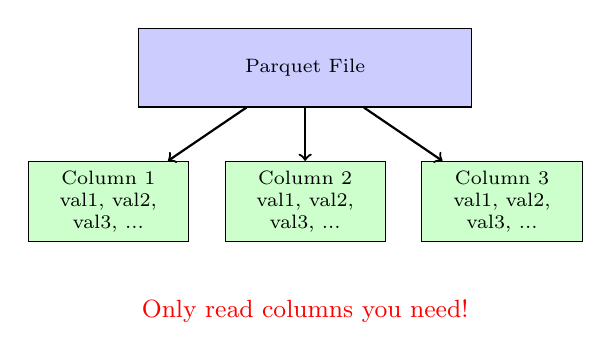
\begin{tikzpicture}[node distance=1.2cm, auto, scale=0.85, every node/.style={font=\scriptsize}]
    % Parquet file box
    \node[draw, rectangle, fill=blue!20, text width=4cm, align=center, minimum height=1cm] (file) at (0,0) {Parquet File};
    
    % Columns - spread out more horizontally
    \node[draw, rectangle, fill=green!20, below of=file, xshift=-2.5cm, yshift=-0.5cm, text width=1.8cm, align=center, minimum height=0.8cm] (c1) {Column 1\\
        val1, val2,\\
        val3, ...};
    \node[draw, rectangle, fill=green!20, below of=file, yshift=-0.5cm, text width=1.8cm, align=center, minimum height=0.8cm] (c2) {Column 2\\
        val1, val2,\\
        val3, ...};
    \node[draw, rectangle, fill=green!20, below of=file, xshift=2.5cm, yshift=-0.5cm, text width=1.8cm, align=center, minimum height=0.8cm] (c3) {Column 3\\
        val1, val2,\\
        val3, ...};
    
    % Note
    \node[below of=c2, yshift=-0.2cm, text width=5cm, align=center, font=\small, text=red] {Only read columns you need!};
    
    % Edges
    \draw[->, thick] (file) -- (c1);
    \draw[->, thick] (file) -- (c2);
    \draw[->, thick] (file) -- (c3);
\end{tikzpicture}
\end{center}
\end{frame}

\begin{frame}[fragile]{Writing Results}
\small
\begin{lstlisting}
# Write to Parquet
df.to_parquet('s3://bucket/output/')

# Write to CSV
df.to_csv('s3://bucket/output/*.csv')

# With options
df.to_parquet(
    's3://bucket/output/',
    compression='snappy',
    write_index=False
)
\end{lstlisting}

\textbf{Key Features:}
\begin{itemize}
    \item Writes partitioned files
    \item One file per partition
    \item Maintains partitioning structure
\end{itemize}
\end{frame}

\begin{frame}[fragile]{Writing Results: Output Structure}
\small
\textbf{Output Structure:}
\begin{verbatim}
output/
+-- part.0.parquet
+-- part.1.parquet
+-- part.2.parquet
+-- part.3.parquet
\end{verbatim}

\vspace{0.2cm}
\textbf{Benefits:}
\begin{itemize}
    \item Each partition is a separate file
    \item Can read back efficiently
    \item Maintains data organization
\end{itemize}
\end{frame}

\begin{frame}{Index Management: Concepts}
\small
\textbf{Index Determines Partitioning:}
\begin{itemize}
    \item Index values determine which partition data goes to
    \item Setting index can be expensive operation
    \item May trigger data shuffle across partitions
\end{itemize}

\vspace{0.2cm}
\textbf{Best Practice:}
\begin{itemize}
    \item Set index during read if possible
    \item Avoid setting index on large datasets unnecessarily
    \item Use \texttt{repartition()} to adjust partition count
\end{itemize}
\end{frame}

\begin{frame}[fragile]{Index Management: Code}
\small
\begin{lstlisting}[basicstyle=\ttfamily\tiny]
# Set index (may trigger shuffle)
df = df.set_index('date')

# Repartition
df = df.repartition(npartitions=8)

# Reset index
df = df.reset_index()
\end{lstlisting}

\vspace{0.2cm}
\textbf{When to Use:}
\begin{itemize}
    \item \texttt{set\_index()}: When you need sorted/indexed access
    \item \texttt{repartition()}: To adjust partition size/count
    \item \texttt{reset\_index()}: To convert index back to column
\end{itemize}
\end{frame}

\begin{frame}[fragile]{When Operations Trigger Computation}
\small
\textbf{Explicit Triggers:}
\begin{itemize}
    \item \texttt{.compute()} - explicit trigger
    \item \texttt{len(df)} - triggers computation
    \item \texttt{df.head()} - triggers partial computation
\end{itemize}

\textbf{Lazy Operations:}
\begin{itemize}
    \item Most operations are lazy
    \item Build task graph only
    \item No data loaded until compute
\end{itemize}

\vspace{0.15cm}
\textbf{Example:}
\begin{lstlisting}
df = dd.read_csv('data/*.csv')  # Lazy
filtered = df[df['col'] > 100]  # Lazy
grouped = filtered.groupby('cat')  # Lazy
result = grouped.sum()  # Lazy
final = result.compute()  # TRIGGERS computation
\end{lstlisting}
\end{frame}

\begin{frame}[fragile]{Memory Management}
\small
\textbf{Key Principles:}
\begin{itemize}
    \item Each partition fits in memory
    \item Operations stream through partitions
    \item \texttt{.persist()} caches in memory
\end{itemize}

\vspace{0.15cm}
\textbf{Example:}
\begin{lstlisting}
# Stream through partitions (low memory)
result = df.groupby('cat').sum().compute()

# Cache in memory (higher memory, faster)
df_persisted = df.persist()
result1 = df_persisted.groupby('cat').sum()
result2 = df_persisted.groupby('cat').mean()
\end{lstlisting}

\textbf{Memory Strategy:}
\begin{itemize}
    \item Default: Stream (low memory)
    \item Use persist: When reusing data (higher memory)
\end{itemize}
\end{frame}

\begin{frame}[fragile]{Performance Tips: Partition Size}
\small
\textbf{Partition Size Guidelines:}
\begin{itemize}
    \item \textbf{Too small}: Overhead dominates (many small tasks)
    \item \textbf{Too large}: Memory issues (partition doesn't fit)
    \item \textbf{Rule of thumb}: 100MB-1GB per partition
\end{itemize}

\vspace{0.1cm}
\textbf{Adjusting Partitions:}
\begin{lstlisting}[basicstyle=\ttfamily\tiny]
# Repartition to different size
df = df.repartition(npartitions=8)  # Fewer, larger partitions
df = df.repartition(npartitions=32)  # More, smaller partitions
\end{lstlisting}

\begin{center}
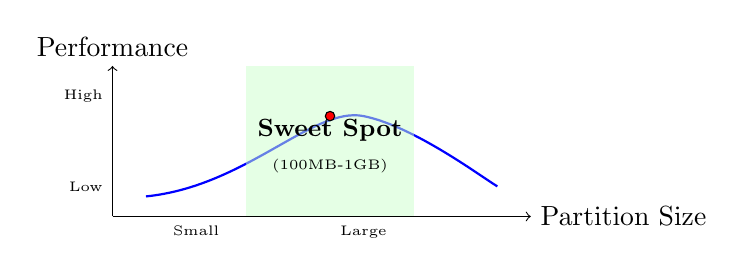
\begin{tikzpicture}[x=2.5cm, y=1.5cm, scale=0.85]
    % Axes
    \draw[->] (0,0) -- (2.5,0) node[right] {Partition Size};
    \draw[->] (0,0) -- (0,1.5) node[above] {Performance};
    
    % Labels
    \node[below] at (0.5,0) {\tiny Small};
    \node[below] at (1.5,0) {\tiny Large};
    \node[left] at (0,0.3) {\tiny Low};
    \node[left] at (0,1.2) {\tiny High};
    
    % Performance curve (inverted U shape)
    \draw[thick, blue] (0.2,0.2) .. controls (0.8,0.3) and (1.2,1.1) .. (1.5,1.0) .. controls (1.8,0.9) and (2.2,0.4) .. (2.3,0.3);
    
    % Sweet spot region
    \fill[green!20, opacity=0.5] (0.8,0) rectangle (1.8,1.5);
    \node[align=center] at (1.3,0.7) {\small\textbf{Sweet Spot}\\\tiny(100MB-1GB)};
    
    % Mark sweet spot
    \draw[fill=red] (1.3,1.0) circle (2pt);
\end{tikzpicture}
\end{center}
\end{frame}

\begin{frame}[fragile]{Performance Tips: Operations}
\small
\textbf{Optimization Strategies:}

\begin{enumerate}
    \item \textbf{Filter early}: Reduces data size
    \begin{lstlisting}[basicstyle=\ttfamily\tiny]
# Good: Filter first
df[df['value'] > 100].groupby('cat').sum()
    \end{lstlisting}

    \item \textbf{Use appropriate dtypes}: Smaller dtypes = less memory
    \begin{lstlisting}[basicstyle=\ttfamily\tiny]
df['id'] = df['id'].astype('int32')
    \end{lstlisting}

    \item \textbf{Avoid iterating over rows}: Use vectorized operations
\end{enumerate}
\end{frame}

\begin{frame}[fragile]{Common Pitfalls: Setting Index}
\small
\begin{lstlisting}
# SLOW: Sets index after loading all data
df = dd.read_parquet('s3://bucket/data/*.parquet')
df = df.set_index('date')  # Expensive shuffle!

# BETTER: Set index during read
df = dd.read_parquet(
    's3://bucket/data/*.parquet',
    index='date'  # Index set during read
)
\end{lstlisting}

\textbf{Why It Matters:}
\begin{itemize}
    \item Setting index requires data shuffle
    \item Can be very expensive for large datasets
    \item Set index during read when possible
\end{itemize}
\end{frame}

\begin{frame}[fragile]{Common Pitfalls: Iterating}
\small
\begin{lstlisting}
# BAD: Iterating over partitions
for partition in df.to_delayed():
    process(partition)

# BETTER: Use vectorized operations
df.apply(func, axis=1)

# BEST: Use built-in operations
df.groupby('cat').apply(func)
\end{lstlisting}

\textbf{Key Principle:}
\begin{itemize}
    \item Avoid Python loops
    \item Use vectorized operations
    \item Leverage Dask's parallelization
\end{itemize}

\vspace{0.15cm}
\textbf{Performance Impact:}
\begin{itemize}
    \item Loops: Sequential, slow
    \item Vectorized: Parallel, fast
\end{itemize}
\end{frame}

\begin{frame}[fragile]{Real-World Example: Flight Data}
\small
\begin{lstlisting}
# Read flight data from S3
df = dd.read_parquet('s3://bucket/flights/*.parquet')

# Filter delayed flights
delayed_flights = df[df['dep_delay'] > 0]

# Group by airline
by_airline = delayed_flights.groupby('carrier').size()

# Compute result
result = by_airline.compute()
\end{lstlisting}

\textbf{Complete Workflow:}
\begin{enumerate}
    \item Read data (lazy)
    \item Filter (lazy)
    \item Group and aggregate (lazy)
    \item Compute (executes everything)
\end{enumerate}
\end{frame}

\begin{frame}{Real-World Example: Execution}
\small
\textbf{What Happens During Compute:}
\begin{itemize}
    \item All operations build task graph
    \item Scheduler optimizes execution
    \item Data processed in parallel
    \item Results combined
\end{itemize}

\vspace{0.2cm}
\textbf{Benefits:}
\begin{itemize}
    \item Efficient: Only reads needed data
    \item Parallel: Processes partitions simultaneously
    \item Scalable: Works with datasets too large for memory
\end{itemize}
\end{frame}

\begin{frame}{Summary}
\small
\textbf{Key Takeaways:}
\begin{itemize}
    \item Dask DataFrame = many pandas DataFrames
    \item Lazy evaluation for efficiency
    \item Pandas-like API (familiar)
    \item Scales to large datasets
\end{itemize}

\vspace{0.1cm}
\textbf{Best Practices:}
\begin{itemize}
    \item Filter early
    \item Right-size partitions
    \item Use persist strategically
    \item Avoid unnecessary index operations
\end{itemize}

\vspace{0.15cm}
\textbf{Next Steps:}
\begin{itemize}
    \item Learn delayed and futures
    \item Explore distributed computing
    \item Practice with real datasets
\end{itemize}
\end{frame}

\end{document}

